\chapter{Probl\`emes sur les lois de conservation}

\section{Changement de direction d'une particule}

\begin{figure}[htb!]
	\begin{center}
		\begin{picture}(150,100)(0,0)
			%axis
			\linethickness{0.05mm}
			\multiput(75,0)(0,10){10}{\line(0,1){8}}
			\multiput(20,50)(7,0){6}{\line(1,0){5}}
			\multiput(100,50)(7,0){6}{\line(1,0){5}}
			%particles
			\put(20,50){\color{black}\circle*{5}}\put(6,47){$m$}
			\put(100,50){\color{black}\circle*{5}}
			%velocities
			\put(20,50){\color{black}\vector(3,1){40}}\put(35,65){$\vec{v}_{1}$}
			\put(100,50){\color{black}\vector(2,1){40}}\put(110,65){$\vec{v}_{2}$}
			%angles
			\linethickness{0.05mm}
			\qbezier(40,50),(40,52),(38,55)
			\put(45,52){$\theta_{1}$}
			\qbezier(115,50),(115,52),(113,55)
			\put(120,52){$\theta_{2}$}
			%potential energies
			\put(25,10){$U_{1}(t_{1})$}
			\put(110,10){$U_{2}(t_{2})$}
		\end{picture}
		\caption{Trajectoire de la particule}\label{FIG:2_1}
	\end{center}
\end{figure}

Par application de la conservation de l'\'energie, nous pouvons \'ecrire :
\benn
	E_{1} = E_{2} \Leftrightarrow \dfrac{m\vec{v_{1}}^{\,2}}{2} + U_{1} = \dfrac{m\vec{v_{2}}^{\,2}}{2} + U_{2}
\eenn
Alors que l'application de la conservation de mouvement suivant l'axe vertical, puisque l'\'energie potentielle est constante suivant cette axe, permet d'\'ecrire :
\benn
	mv_{1}\sin(\theta_{1}) = mv_{2}\sin(\theta_{2}) \Leftrightarrow v_{2} = v_{1}\dfrac{\sin(\theta_{1})}{\sin(\theta_{2})}
\eenn
En reprenant la conservation de l'\'energie, nous avons ainsi :
\bea
	\dfrac{m\vec{v_{1}}^{\,2}}{2} + U_{1} & = & \dfrac{m\vec{v_{2}}^{\,2}}{2} + U_{2} \Leftrightarrow \dfrac{mv_{1}^{2}}{2} + U_{1} = \dfrac{mv_{2}^{2}}{2} + U_{2} \nonumber \\
	\Leftrightarrow \dfrac{mv_{1}^{2}}{2} + U_{1} & = & \dfrac{mv_{1}^{2}\sin^{2}(\theta_{1})}{2\sin^{2}(\theta_{2})} + U_{2} \Leftrightarrow \dfrac{mv_{1}^{2}}{2}\left(\dfrac{\sin^{2}(\theta_{1})}{\sin^{2}(\theta_{2})} - 1\right) = U_{1} - U_{2} \nonumber \\
	\Leftrightarrow \dfrac{\sin(\theta_{1})}{\sin(\theta_{2})} & = & \sqrt{1 + 2\dfrac{U_{1} - U_{2}}{mv_{1}^{2}}} \label{EQ:7_EX1_1}
\eea
dont une repr\'esentation est disponible sur la figure (\ref{FIG:2_EX2}).

\begin{figure}[htb!]
	\begin{center}
		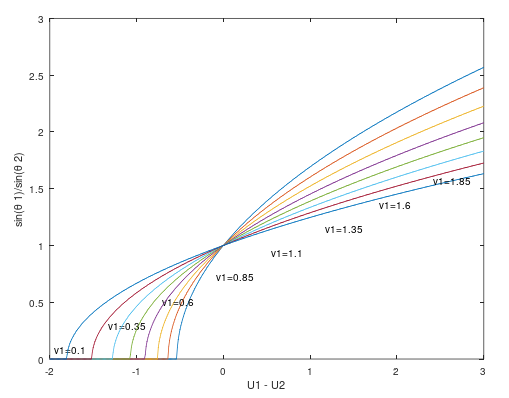
\includegraphics[width=10cm]{chapter_02_exercice_2}
		\caption{\'Evolution du rapport $\dfrac{\sin(\theta_{1})}{\sin(\theta_{2})}$ en fonction de $U_{1} - U_{2}$ pour $m = 1$}\label{FIG:2_EX2}
	\end{center}
\end{figure}

\section{Transformation de l'action d'un r\'ef\'erentiel galil\'een \`a un autre}

Le passage d'un r\'ef\'erentiel galil\'een \`a un autre s'op\`ere tel que, voir \'equation (\ref{EQ:3_3}):
\benn
	\vec{r} = \vec{r'} + \vec{V}\mathrm{t} \Leftrightarrow \vec{v} = \vec{v'} + \vec{V}
\eenn
La fonction de Lagrange devient :
\bea
	L & = & T - U = \sum_{a=1}^{s}\dfrac{m_{a}\vec{v}_{a}^{\,2}}{2} - U(\begin{Bmatrix}\vec{r}_{a}\end{Bmatrix}^{s}_{1}) \nonumber \\
	& = & \sum_{a}\dfrac{m_{a}\vec{v'}_{a}^{\,2}}{2} + \sum_{a}\dfrac{m_{a}\vec{V}^{\,2}}{2} + \sum_{a}m_{a}\vec{v'}_{a}\cdot\vec{V} - U \nonumber \\
	& = & \sum_{a}\dfrac{m_{a}\vec{v'}_{a}^{\,2}}{2} - U + \vec{V}\cdot\sum_{a}m_{a}\vec{v'}_{a} + \vec{V}^{\,2}\sum_{a}\dfrac{m_{a}}{2} \nonumber
\eea
ce qui peut aussi s'\'ecrire :
\benn
	L = L' + \vec{V}\cdot\vec{P'} + \dfrac{1}{2}\mu\vec{V}^{\,2}
\eenn
Ce qui implique pour l'action du syst\`eme : 
\benn
	S = \int L\mathrm{dt} = \int L'\mathrm{dt} + \vec{V}\cdot\int\vec{P'}\mathrm{dt} + \dfrac{1}{2}\mu\vec{V}^{\,2}\int \mathrm{dt}
\eenn
or l'\'equation (\ref{EQ:8_3}) donne pour la d\'efinition du centre d'inertie :
\benn
	\vec{R} = \dfrac{\sum_{a}m_{a}\vec{r}_{a}}{\sum_{a}m_{a}}
\eenn
En d\'erivant par le temps l'expression pr\'ec\'edente :
\benn
	\mu\dfrac{\vec{R}}{\mathrm{dt}} = \sum_{a}m_{a}\dfrac{\mathrm{d}\vec{r}_{a}}{\mathrm{dt}} = \sum_{a}m_{a}\vec{v}_{a} = \vec{P}
\eenn
Donc l'action devient :
\benn
	S = S' + \vec{V}\cdot\int\mu\dfrac{\vec{R'}}{\mathrm{dt}}\mathrm{dt} + \dfrac{1}{2}\mu\vec{V}^{\,2}\mathrm{t} = S' + \mu\vec{V}\cdot\vec{R'} + \dfrac{1}{2}\mu\vec{V}^{\,2}\mathrm{t}
\eenn

\section{Exercices sur le moment cin\'etique}

\subsection{En coordonn\'ees cylindriques}

Pour un point mat\'eriel de masse $m$ :
\bea
	\vec{M} & = & \vec{r}\wedge\vec{P} \nonumber \\
	& = & \begin{pmatrix} r\cos\varphi \\ r\sin\varphi \\ z \end{pmatrix} \wedge m \begin{pmatrix} -r\sin\varphi\dot{\varphi} + \dot{r}\cos\varphi \\ r\cos\varphi\dot{\varphi} + \dot{r}\sin\varphi \\ \dot{z} \end{pmatrix} \nonumber \\
	& = & m \begin{pmatrix} r\sin\varphi\dot{z} - z(r\cos\varphi\dot{\varphi} + \dot{r}\sin\varphi) \\ -r\cos\varphi\dot{z} + z(\dot{r}\cos\varphi - r\sin\varphi\dot{\varphi}) \\ r^{2}\cos^{2}\varphi\dot{\varphi} + r\dot{r}\cos\varphi\sin\varphi + r^{2}\sin^{2}\varphi\dot{\varphi} - r\dot{r}\cos\varphi\sin\varphi \end{pmatrix} \nonumber \\
	\begin{pmatrix} M_{x} \\ M_{y} \\ M_{z} \end{pmatrix} & = & m \begin{pmatrix} \sin\varphi(r\dot{z} - \dot{r}z) - rz\cos\varphi\dot{\varphi} \\ -\cos\varphi(r\dot{z} - \dot{r}z) - rz\sin\varphi\dot{\varphi} \\ r^{2}\dot{\varphi} \end{pmatrix} \nonumber
\eea
pour arriver à la norme au carr\'e :
\bea
	\parallel \vec{M} \parallel^{2} & = & M_{x}^{2} + M_{y}^{2} + M_{z}^{2} \nonumber \\
	& = & m^{2}(\sin^{2}\varphi(r\dot{z} - \dot{r}z)^{2} + r^{2}z^{2}\cos^{2}\varphi\dot{\varphi}^{2} - 2rz(r\dot{z} - \dot{r}z)\cos\varphi\sin\varphi\dot{\varphi} \nonumber \\
	& + & \cos^{2}\varphi(r\dot{z} - \dot{r}z)^{2} + r^{2}z^{2}\sin^{2}\varphi\dot{\varphi}^{2} + 2rz(r\dot{z} - \dot{r}z)\cos\varphi\sin\varphi\dot{\varphi} + r^{4}\dot{\varphi}^{2} \nonumber \\
	M^{2} & = & m^{2}(r\dot{z} - \dot{r}z)^{2} + m^{2}r^{2}\dot{\varphi}^{2}(r^{2} + z^{2}) \nonumber
\eea

\subsection{En coordonn\'ees sph\'eriques}

Pour un point mat\'eriel de masse $m$ :
\bea
	\vec{M} & = & \vec{r}\wedge\vec{P} \nonumber \\
	& = & \begin{pmatrix} r\sin\theta\cos\varphi \\ r\sin\theta\sin\varphi \\ r\cos\theta \end{pmatrix} \wedge m \begin{pmatrix} \dot{r}\sin\theta\cos\varphi + r\cos\theta\cos\varphi\dot{\theta} - r\sin\theta\sin\varphi\dot{\varphi} \\ \dot{r}\sin\theta\sin\varphi + r\cos\theta\sin\varphi\dot{\theta} - r\sin\theta\cos\varphi\dot{\varphi} \\ \dot{r}\cos\theta + r\sin\theta\dot{\theta} \end{pmatrix} \nonumber \\
	& = & m \begin{pmatrix} r\dot{r}\cos\theta\sin\theta\sin\varphi - r^{2}\sin^{2}\theta\sin\varphi\dot{\theta} - r\dot{r}\cos\theta\sin\theta\sin\varphi \\ r\dot{r}\cos\theta\sin\theta\cos\varphi + r^{2}\cos^{2}\theta\cos\varphi\dot{\theta} - r\dot{r}\cos\theta\sin\theta\cos\varphi \\ r\dot{r}\sin^{2}\theta\cos\varphi\sin\varphi + r^{2}\cos\theta\sin\theta\cos\varphi\sin\varphi\dot{\theta} + r^{2}\sin^{2}\theta\cos^{2}\varphi\dot{\varphi} \end{pmatrix} \nonumber \\
	& + & m \begin{pmatrix} -r^{2}\cos^{2}\theta\sin\varphi\dot{\theta} - r^{2}\cos\theta\sin\theta\cos\varphi\dot{\varphi} \\ r^{2}\sin^{2}\theta\cos\varphi\dot{\theta} - r^{2}\cos\theta\sin\theta\sin\varphi\dot{\varphi} \\ -r\dot{r}\sin^{2}\theta\cos\varphi\sin\varphi - r^{2}\cos\theta\sin\theta\cos\varphi\sin\varphi\dot{\theta} + r^{2}\sin^{2}\theta\sin^{2}\varphi\dot{\varphi} \end{pmatrix} \nonumber \\
	& = & m \begin{pmatrix} -r^{2}\sin\varphi\dot{\theta} - r^{2}\cos\theta\sin\theta\cos\varphi\dot{\varphi} \\ r^{2}\cos\varphi\dot{\theta} - r^{2}\cos\theta\sin\theta\cos\varphi\dot{\varphi} \\ r^{2}\sin^{2}\theta\dot{\varphi} \end{pmatrix} \nonumber
\eea
Cela donne pour la norme au carr\'e :
\bea
	\parallel \vec{M} \parallel^{2} & = & m^{2} ( r^{4}\sin^{2}\varphi\dot{\theta}^{2} + r^{4}\cos^{2}\theta\sin^{2}\theta\cos^{2}\dot{\varphi}^{2} + 2r^{4}\cos\theta\sin\theta\cos\varphi\sin\varphi\dot{\theta}\dot{\varphi} \nonumber \\
	& + & r^{4}\cos^{2}\varphi\dot{\theta}^{2} + r^{4}\cos^{2}\theta\sin^{2}\theta\sin^{2}\dot{\varphi}^{2} - 2r^{4}\cos\theta\sin\theta\cos\varphi\sin\varphi\dot{\theta}\dot{\varphi} \nonumber \\
	& + & r^{4}\sin^{4}\theta\dot{\varphi}^{2} ) \nonumber \\
	& = & m^{2} ( r^{4}\dot{\theta}^{2} + r^{4}\cos^{2}\theta\sin^{2}\theta\dot{\varphi}^{2} + r^{4}\sin^{4}\theta\dot{\varphi}^{2} ) \nonumber
\eea
Soit finalement :
\benn
	M^{2} = m^{2}r^{4} (\dot{\theta}^{2} + sin^{2}\theta\dot{\varphi}^{2})
\eenn

\subsection{Conservation de l'impulsion et du moment cin\'etique dans des cas particuliers}

Dans cette s\'erie d'exemples, cela consiste \`a appliquer l'invariance de la fonction de Lagrange lors d'une rotation et/ou d'une translation pour d\'eterminer quelles composantes se conservent. Ainsi :
\begin{itemize}
	\item[a)] avec champ issu d'un plan homog\`ene d\'efini par $(x,y)$, l'invariance lors d'une translation permet de conclure \`a la conservation de $P_{x}$ et $P_{y}$ alors que l'invariance lors d'une rotation ne peut conserver que $M_{z}$ ;
	\item[b)] avec champ issu d'un cylindre homog\`ene autour de l'axe $z$, l'invariance lors d'une translation ne permet de conclure qu'\`a la conservation de $P_{z}$ alors que l'invariance lors d'une rotation ne peut conserver que $M_{z}$ ;
	\item[c)] avec champ issu d'un prisme homog\`ene infini suivant l'axe $z$, l'invariance lors d'une translation permet de conclure \`a la conservation de $P_{x}$ et $P_{y}$ alors qu'il n'y a pas d'axe de rotation permettant une rotation infinit\'esimale possible et une invariance de la fonction de Lagrange ;
	\item[d)] avec champ issu de points, seule l'invariance lors d'une rotation autour de l'axe d\'efini par la droite passant par les deux points peut conserver la projection du moment cin\'etique sur cette axe ;
	\item[e)] avec champ issu d'un demi-plan homog\`ene d\'efini par $(x,y > 0)$, l'invariance lors d'une translation permet de conclure \`a la conservation de $P_{y}$ alors que l'invariance lors d'une rotation ne peut conserver que $M_{z}$ ;
	\item[f)] avec champ issu d'un c\^one homog\`ene suivant l'axe $z$, seule l'invariance lors d'une rotation autour de l'axe $z$ peut conserver $M_{z}$ ;
	\item[g)] avec champ issu d'un tore circulaire homog\`ene dont l'axe est $z$, seule l'invariance lors d'une rotation autour de l'axe $z$ peut conserver $M_{z}$ ;
	\item[h)] avec champ issu d'une h\'elice cylindrique homog\`ene et infinie suivant l'axe $z$ dont le pas est $h$. L'invariance de la fonction de Lagrange est possible selon un d\'eplacement issu d'une rotation d'angle $\delta\varphi$ autour de l'axe $z$ et d'une translation simultan\'ee le long de $z$ de $\delta z = \dfrac{h}{2\pi}\delta\varphi$. Par d\'efinition :
		\benn
			\delta L = \dfrac{\partial L}{\partial z}\delta z + \dfrac{\partial L}{\partial\varphi}\delta\varphi = \dot{P}_{z}\delta z + \dot{M}_{z}\delta\varphi
		\eenn
		car l'\'equation (\ref{EQ:7_7}) a donn\'e $\dot{p}_{i} = \dfrac{\partial L}{\partial q_{i}}$ et l'\'equation (\ref{EQ:9_7}) que $M_{z} = \dfrac{\partial L}{\partial\dot{\varphi}}$. Ce qui implique que $\dot{M}_{z} = \dfrac{d}{\mathrm{dt}}\left(\dfrac{\partial L}{\partial\dot{\varphi}}\right) = \dfrac{\partial L}{\partial\varphi}$ selon les \'equations de Lagrange (\ref{EQ:2_6}). Et on en vient \`a :
		\benn
			\forall \delta\varphi\text{, }\delta L = \delta\varphi\left(\dfrac{h}{2\pi}\dot{P}_{z} + \dot{M}_{z}\right)
		\eenn
		soit $\delta L = 0$ si et seulement si :
		\benn
			\dfrac{h}{2\pi}\dot{P}_{z} + \dot{M}_{z} = 0
		\eenn
		ou encore, par int\'egration par rapport au temps :
		\benn
			\dfrac{h}{2\pi}P_{z} + M_{z} = Cste
		\eenn
\end{itemize}

\section{Similitudes m\'ecaniques}

\subsection{Cas de deux masses diff\'erentes}

Les deux points mat\'eriels ont la m\^eme \'energie potentielle et se d\'eplacent sur des trajectoires identiques. Aussi la fonction de Lagrange est identique pour les deux points mat\'eriels, soit $L = T - U = L' = T' - U'$. Sachant que $U=U'$, cela implique :
\bea
	T & = & T' \Leftrightarrow \dfrac{1}{2}mv^{2} = \dfrac{1}{2}m'v'^{2} \Leftrightarrow \dfrac{m'}{m} = \left(\dfrac{v}{v'}\right)^{2} \nonumber \\
	\Leftrightarrow \dfrac{m'}{m} & = & \left(\dfrac{l\mathrm{t}'}{\mathrm{t}l'}\right)^{2} \Leftrightarrow \dfrac{m'}{m} = \left(\dfrac{\mathrm{t}'}{\mathrm{t}}\right)^{2} \Leftrightarrow \dfrac{\mathrm{t}'}{\mathrm{t}} = \sqrt{\dfrac{m'}{m}} \nonumber
\eea
car $l=l'$ (trajectoires identiques).

\subsection{Cas d'une \'energie potentielle vari\'ee}

\'Etudions le cas d'une trajectoire identique avec $U' = \alpha U$. L'invariance de la fonction de Lagrange peut s'\'ecrire :
\benn
	\delta T = \delta U \Leftrightarrow \left(\dfrac{v'}{v}\right)^{2} = \dfrac{U'}{U} \Leftrightarrow \left(\dfrac{l'\mathrm{t}}{\mathrm{t}'l}\right)^{2} = \dfrac{U'}{U} \Leftrightarrow \dfrac{\mathrm{t}'}{\mathrm{t}} = \sqrt{\dfrac{U}{U'}}
\eenn
car $l=l'$ (trajectoires identiques).